\chapter*{Summary}
\addcontentsline{toc}{chapter}{Summary}

\noindent 
\dropcap{T}{his} summary is written especially for
non-biologists, so they can understand what is
discussed in this thesis.

\paragraph{Speciation}

There are plenty of (animal, plant, etc.) species on the world.
In Earth's early days this was not yet the the case:
it took hundreds of millions of years for the first species to arise.
In the many years that followed, billions of species have formed.
The process that creates new species, we call speciation.

\paragraph{Speciation in bacteria}

There are multiple ways that speciation can occur.
For bacteria, we state that two bacteria are of different species,
if their DNA differs enough. Bacteria multiply when the 
environment is suitable and with each cell division, the DNA
of the new bacteria changes slightly. 
Thus, when one starts with two identical bacteria, 
after some time, one
ends up with two different bacterial species.

\paragraph{Speciation in animals}

For animals it is harder to state when two animals are of two 
different species. A commonly used definition is that two groups
of animals are of different species, when the offspring 
of individuals of the different groups is either absent 
or results in infertile grandchildren.

There are multiple mechanisms that cause speciation in animals.
One simple mechanisms is the split of group in two groups
by a change in the environment, as can be done by a river
or a mountain.

\paragraph{Phylogenies}

When we look at multiple species over a longer period of 
time (that is, millions of years!), likely there will be speciation
events. Some species will give rise to more new species than others.
We can display this process using a phylogenetic tree, as shown
in figure \ref{fig:phylogeny}.

\begin{figure}
  \centering
  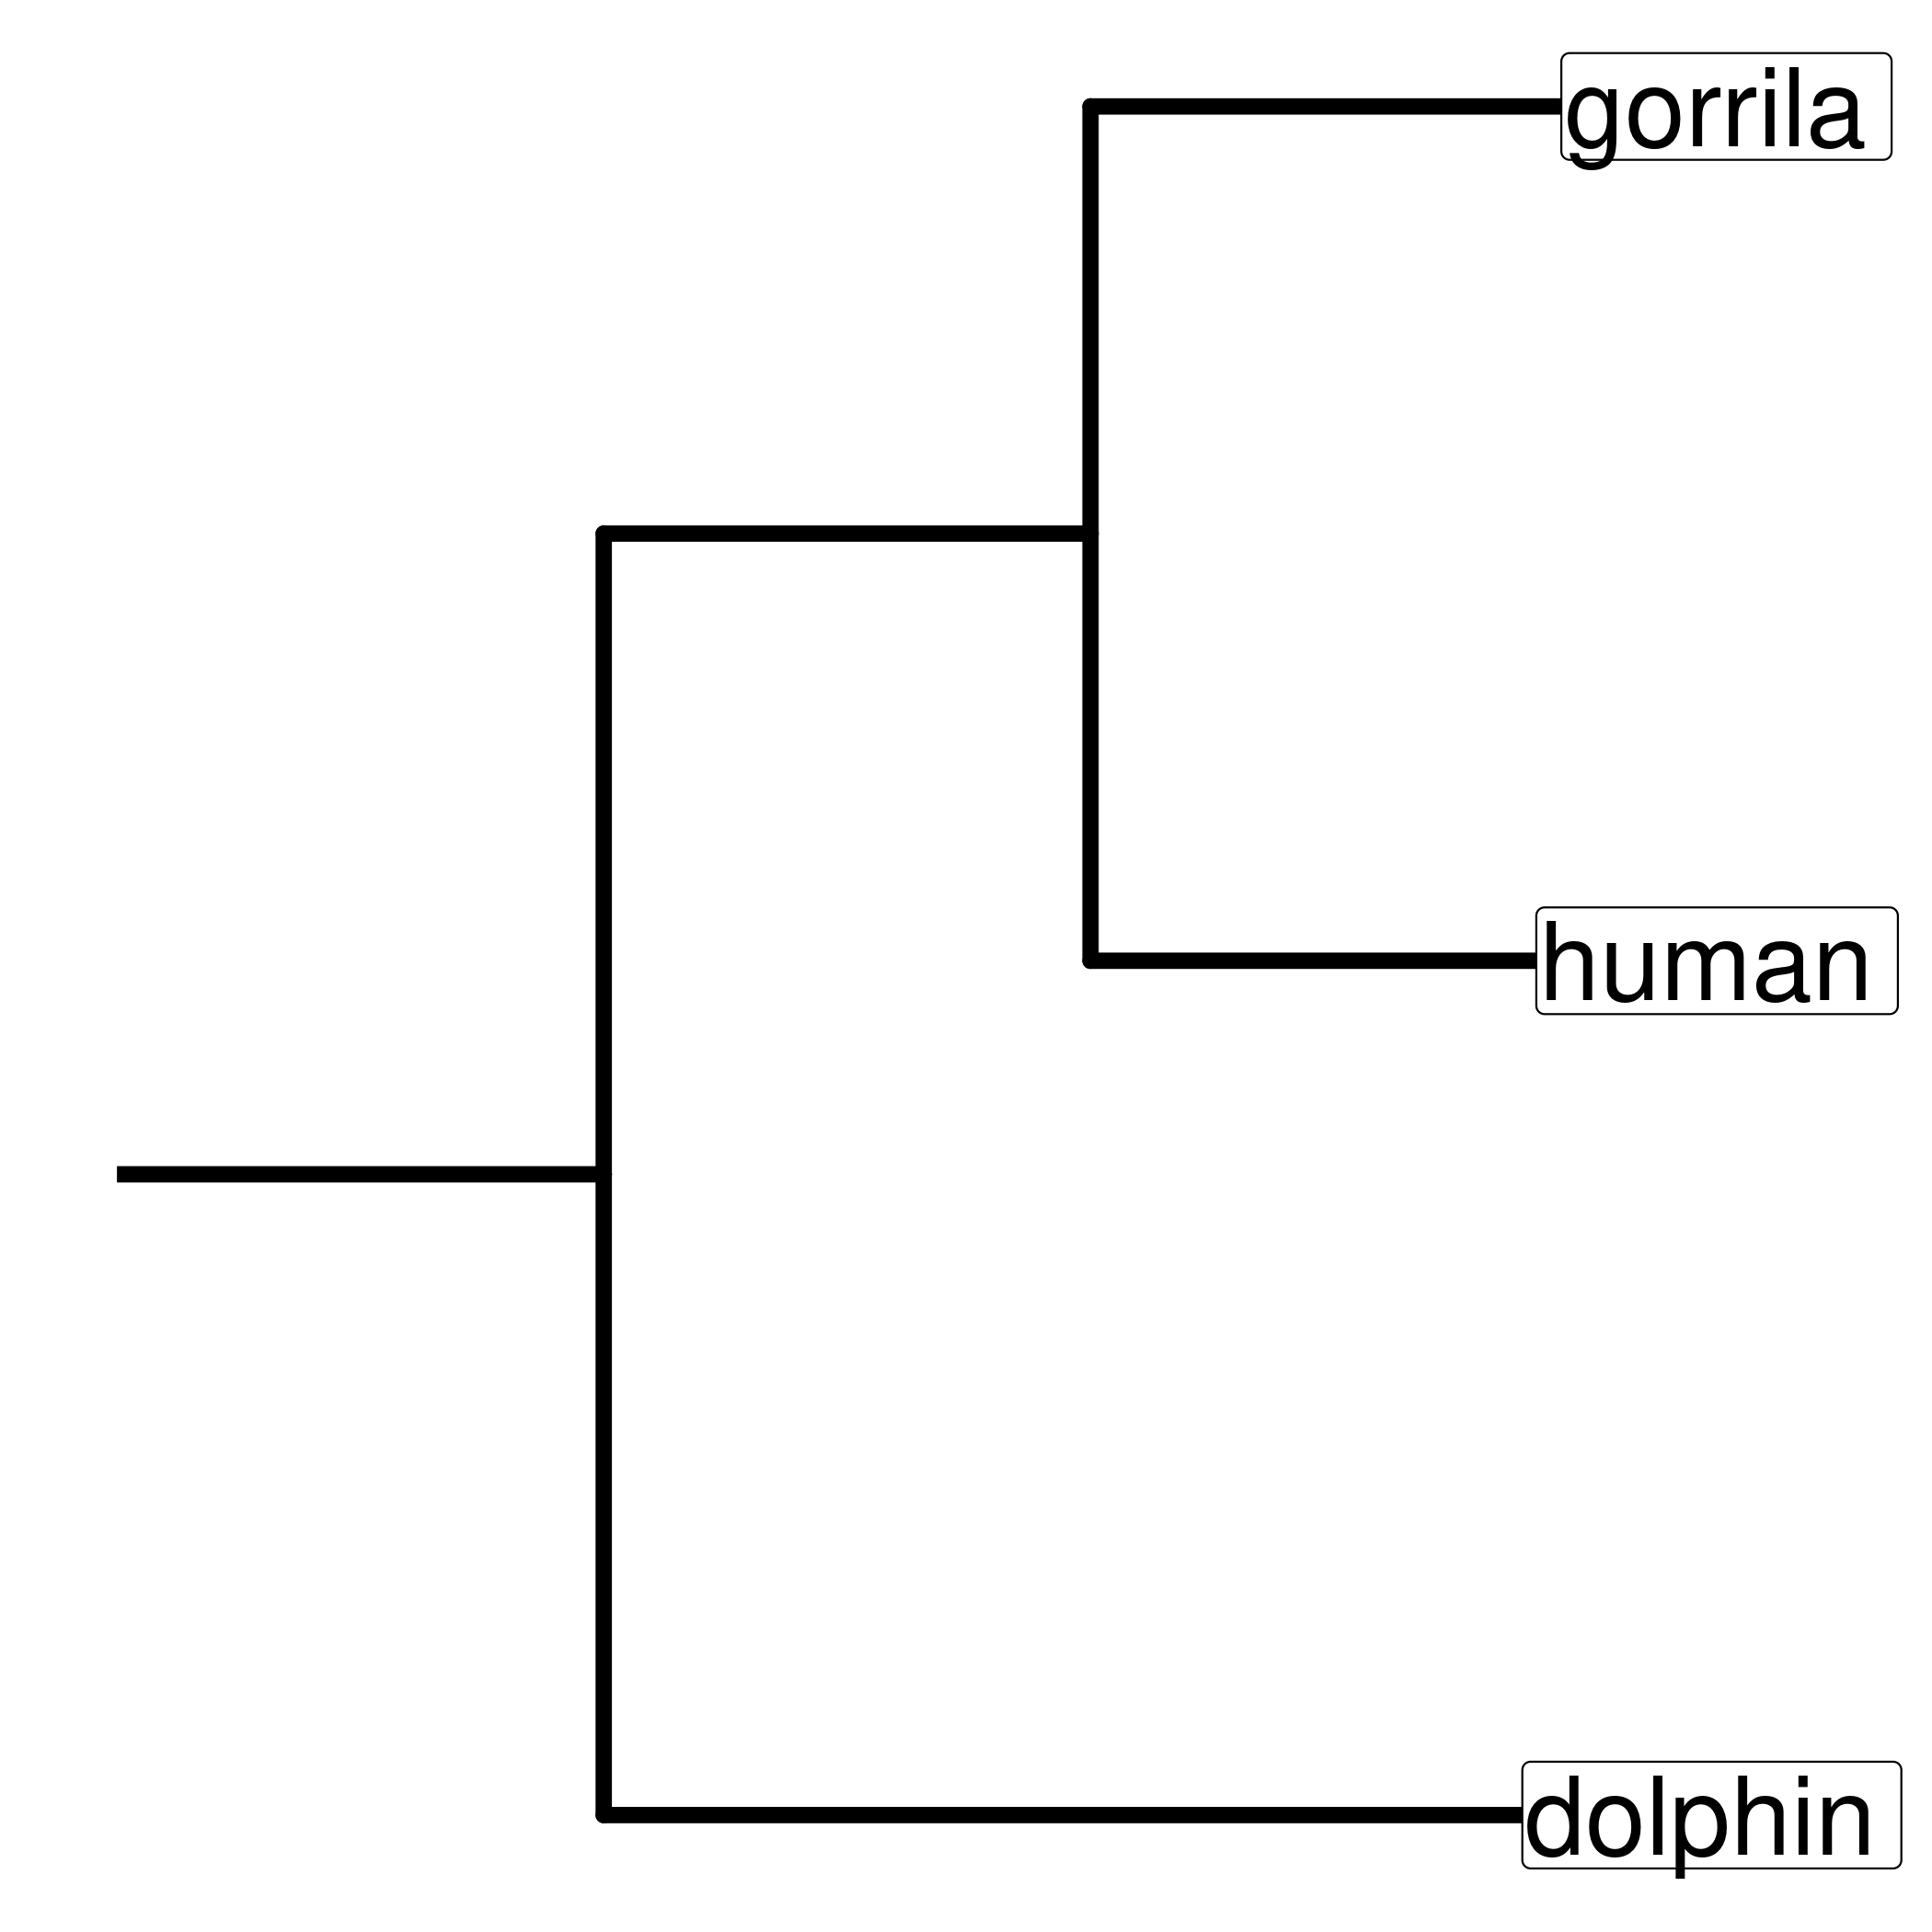
\includegraphics[width=0.5\textwidth]{phylogeny.png}
  \caption{
    A phylogeny that displays that human's and gorilla's
    are more related to one another, compared to
    humans and dolphins.
    This phylogeny is not to scale.
  }
  \label{fig:phylogeny}
\end{figure}

\paragraph{DNA}

One needs some form of information to base a phylogeny on,
such as, for example, the DNA sequence of the species
within the phylogeny.
All living beings have DNA, thanks to which it is possible 
to put all species in one big phylogeny.
Each time DNA is transferred to a next generation, it
changes a little bit.
Due to this property, it is possible to base a phylogeny
on DNA sequences.
Simply put: species that have a more similar DNA sequence, are
closer related.

\paragraph{Phylogenetic model}

There are multiple ways to construct a phylogeny
from DNA sequences, because one can have different 
assumptions regarding how speciation occurs.
For example, one can assume that speciation events
occur just as often all the time (on average) in all species.
Or one may assume that DNA of all species have the same mutation rate.
The collection of assumptions, we call a model. In this case,
we call it a phylogenetic model.

\paragraph{Constructing phylogenies}

There are computer programs that construct a phylogeny from a
phylogenetic model and DNA sequences.
One of the most popular of such programs is called BEAST2.
Because I would simulate many thousands of phylogenies,
I needed to be able to do so from scripts only (that is,
without any mouse clicks). For that reasons, I programmed
\verb;babette;, an R package with which one can call BEAST2.
In chapter 2, one can read more about \verb;babette;.

\paragraph{Phylogenetic models}

Because one can pick many different assumption regarding speciation,
the question which one is best arises quickly.
And there are also multiple methods to compare 
phylogenetic models (that is, to find out which one is 'best').
A drawback of most methods is that the phylogenetic model
needs to be understood well mathematically.
This means, that before one can measure how 'good' a new
phylogenetic model is, it needs to be solved mathematically first.

\paragraph{Determine how good phylogenetic models are}

Giovanni, Rampal and I invented a way to determine if
it is important to solve a new phylogenetic model analytically.
With our new method, one only needs to simulate a lot
of phylogenies using the novel method.
Usually, this is way easier than solving a model mathematically.
This method was put in an R package called \verb;pirouette;. 
In chapter 3 one can read more about \verb;pirouette;.

\paragraph{Testing a new speciation model}

After we invented a method to determine how important it is
to solve a phylogenetic model mathematically, we applied
the method on a new phylogenetic model that has not yet been
solved mathematically.

This new model is named the MBD ('Multiple-Birth Death') model
and was invented by Giovanni.
In this model, one assumes that speciation occurs in all species
equally often on average, except that sometimes 
a 'speciation wave' occurs, in which multiple species speciate
at the same time. In chapter 4 one can read how we did this exactly.

We found out, that would nature follow the MBD model, we
can make phylogenies using simpler models that are just as good.

\paragraph{Conclusion}

This thesis shows that we can find out whether or not we should investigate
a novel phylogenetic model in-dept, so that scientists can better
spend their time.

The nice thing about my research is that other scientists also profit
from it: with \verb;babette; anyone can easily constrict phylogenies
from DNA sequences. At the moment of writing, there have been 
3 scientific publications that use \verb;babette;.
Also \verb;pirouette; has become a strong R package, but 
without any citations yet.

